% !TeX root = ../main.tex

\chapter{系统测试}

系统测试的目的是将系统的功能实现与需求设计进行比较,发现系统中存在
的不满足用户需求的情况或者程序中存在的问题,从而对系统功能进行改进,
提高软件的可靠性。本章主要针对系统各模块的功能测试和性能测试进行介绍\cite{32}。

功能测试我们使用的是Swagger,Swagger是一种RESTful API文档生成工具,
它可以帮助开发者更方便地描述、调用和测试API。使用Swagger可以自动生成API文档,
并提供一个交互式的UI界面,方便开发者查看和测试API接口。除此之外,Swagger还提供了许多有用的功能,
例如自动生成客户端SDK、自动生成API测试代码、集成Mock数据等。

性能测试我们使用的是JMeter,JMeter是一个开源的性能测试工具,它可以用于测试Web应用程序、
Web服务、FTP、数据库、消息队列等各种应用程序的性能。JMeter支持多线程测试,
可以模拟大量用户同时访问应用程序,以评估应用程序的性能和稳定性。
JMeter还提供了各种图表和报告来帮助用户分析和解释测试结果。
JMeter具有简单易用的界面,用户可以通过图形化界面或脚本方式进行测试。

\section{数据源管理模块}

在数据源页面,我们可以看到所有已创建的数据源,然后我们还可以对数据源进行创建、查看、编辑、删除功能,
支持的数据源有关系型数据库Mysql,消息队列数据源Tube、Kafka、Pulsar等数据源。
这里我们仅展示创建MySQL数据源、获取数据源列表、测试数据源连通性的接口测试。

创建Mysql数据源的接口测试如表\ref{tab:exampletable1}所示:

\begin{table}[H]
  \centering
  \caption{创建Mysql数据源接口测试}
  \label{tab:exampletable1}
  \begin{tabular}{ll}
    \toprule
    接口描述         & 创建Mysql数据源          \\
    \midrule
    测试类型         & 功能测试         \\
    前置条件         & 后端服务器、MySQL服务器正常         \\
    接口地址       & /formation/v1/datasource/createKafkaDatasource         \\
    请求方式         & POST      \\
    请求数据类型         & application/json     \\
    响应数据类型         & application/json,*/*           \\
    实际结果         & 达到预期结果           \\
    结论            & 测试通过           \\
    \bottomrule
  \end{tabular}
\end{table}

获取数据源列表的接口测试如表\ref{tab:exampletable2}所示:

\begin{table}[H]
  \centering
  \caption{获取数据源列表接口测试}
  \label{tab:exampletable2}
  \begin{tabular}{ll}
    \toprule
    接口描述         & 获取数据源列表         \\
    \midrule
    测试类型         & 功能测试         \\
    前置条件         & 后端服务器、MySQL服务器正常         \\
    接口地址       & /formation/v1/datasource/getDatasourceList         \\
    请求方式         & GET      \\
    请求数据类型         & application/json     \\
    响应数据类型         & application/json,*/*           \\
    实际结果         & 达到预期结果           \\
    结论            & 测试通过           \\
    \bottomrule
  \end{tabular}
\end{table}

测试数据源连通性的接口测试如表\ref{tab:exampletable3}所示:

\begin{table}[H]
  \centering
  \caption{测试数据源连通性接口测试}
  \label{tab:exampletable3}
  \begin{tabular}{ll}
    \toprule
    接口描述         & 测试数据源连通性         \\
    \midrule
    测试类型         & 功能测试         \\
    前置条件         & 后端服务器、MySQL服务器正常         \\
    接口地址       & /formation/v1/datasource/testConnectivity         \\
    请求方式         & POST      \\
    请求数据类型         & application/json     \\
    响应数据类型         & application/json,*/*           \\
    实际结果         & 达到预期结果           \\
    结论            & 测试通过           \\
    \bottomrule
  \end{tabular}
\end{table}

\section{元数据管理模块}

元数据是管理Iceberg表元数据的,在元数据页面,我们可以查看已创建的库表,还可以关联
自己在别处创建的Iceberg表元数据,还可以查看和编辑已创建的Iceberg表,还有数据优化也是在
元数据管理中配置的。相关的的测试如下:

创建Iceberg表的接口测试如表\ref{tab:exampletable4}所示:

\begin{table}[H]
  \centering
  \caption{创建Iceberg表接口测试}
  \label{tab:exampletable4}
  \begin{tabular}{ll}
    \toprule
    接口描述         & 创建Iceberg表         \\
    \midrule
    测试类型         & 功能测试         \\
    前置条件         & 后端服务器、MySQL服务器、Hive Metastore服务正常         \\
    接口地址       & /formation/v1/metadata/createTable        \\
    请求方式         & POST      \\
    请求数据类型         & application/json     \\
    响应数据类型         & application/json,*/*           \\
    实际结果         & 达到预期结果           \\
    结论            & 测试通过           \\
    \bottomrule
  \end{tabular}
\end{table}

关联已有表的接口测试如表\ref{tab:exampletable5}所示:

\begin{table}[H]
  \centering
  \caption{关联已有表接口测试}
  \label{tab:exampletable5}
  \begin{tabular}{ll}
    \toprule
    接口描述         & 关联已有表         \\
    \midrule
    测试类型         & 功能测试         \\
    前置条件         & 后端服务器、MySQL服务器、Hive Metastore服务正常         \\
    接口地址       & /formation/v1/metadata/associateTable        \\
    请求方式         & POST      \\
    请求数据类型         & application/json     \\
    响应数据类型         & application/json,*/*           \\
    实际结果         & 达到预期结果           \\
    结论            & 测试通过           \\
    \bottomrule
  \end{tabular}
\end{table}

注册数据库接口测试如表\ref{tab:exampletable6}所示:

\begin{table}[H]
  \centering
  \caption{注册数据库接口测试}
  \label{tab:exampletable6}
  \begin{tabular}{ll}
    \toprule
    接口描述         & 注册数据库到数据湖         \\
    \midrule
    测试类型         & 功能测试         \\
    前置条件         & 后端服务器、MySQL服务器、Hive Metastore服务正常         \\
    接口地址       & /formation/v1/metadata/registerDatabase        \\
    请求方式         & POST      \\
    请求数据类型         & application/json     \\
    响应数据类型         & application/json,*/*           \\
    实际结果         & 达到预期结果           \\
    结论            & 测试通过           \\
    \bottomrule
  \end{tabular}
\end{table}

获取表列表测试用例如表\ref{tab:exampletable7}所示:

\begin{table}[H]
  \centering
  \caption{获取表列表接口测试}
  \label{tab:exampletable7}
  \begin{tabular}{ll}
    \toprule
    接口描述         & 获取指定库下的表         \\
    \midrule
    测试类型         & 功能测试         \\
    前置条件         & 后端服务器、MySQL服务器、Hive Metastore服务正常         \\
    接口地址       & /formation/v1/metadata/getTableList        \\
    请求方式         & GET      \\
    请求数据类型         & application/json     \\
    响应数据类型         & application/json,*/*           \\
    实际结果         & 达到预期结果           \\
    结论            & 测试通过           \\
    \bottomrule
  \end{tabular}
\end{table}

获取数据库列表接口测试如表\ref{tab:exampletable8}所示:

\begin{table}[H]
  \centering
  \caption{获取数据库列表接口测试}
  \label{tab:exampletable8}
  \begin{tabular}{ll}
    \toprule
    接口描述         & 从安全中心获取数据库列表         \\
    \midrule
    测试类型         & 功能测试         \\
    前置条件         & 后端服务器、MySQL服务器、Hive Metastore服务正常         \\
    接口地址       & /formation/v1/metadata/getDatabaseList        \\
    请求方式         & GET      \\
    请求数据类型         & application/json     \\
    响应数据类型         & application/json,*/*           \\
    实际结果         & 达到预期结果           \\
    结论            & 测试通过           \\
    \bottomrule
  \end{tabular}
\end{table}

\section{数据入湖模块}

数据入湖模块是管理入湖任务的,任务分为两种:实时入湖和存量入湖,
两种任务都需要填写基础信息、源表、目标表、参数及资源。在数据入湖页面,我们可以查看已创建的任务,
也可以创建新的入湖任务或者进行编辑和删除;点击详情可以跳转到不同的平台查看任务的运行状态,存量入湖任务会到US统一调度平台查看任务,
实时入湖任务会到Oceanus实时处理平台查看任务。相关的测试如下:

创建实时任务接口测试如表\ref{tab:exampletable9}所示:

\begin{table}[H]
  \centering
  \caption{创建实时任务接口测试}
  \label{tab:exampletable9}
  \begin{tabular}{ll}
    \toprule
    接口描述         & 创建实时入湖任务         \\
    \midrule
    测试类型         & 功能测试         \\
    前置条件         & 后端服务器、MySQL服务器、Hive Metastore服务、Oceanus平台正常         \\
    接口地址       & /formation/v1/tasks/streaming/createJob        \\
    请求方式         & POST      \\
    请求数据类型         & application/json     \\
    响应数据类型         & application/json,*/*           \\
    实际结果         & 达到预期结果           \\
    结论            & 测试通过           \\
    \bottomrule
  \end{tabular}
\end{table}

创建存量入湖任务接口测试如表\ref{tab:exampletable10}所示:

\begin{table}[H]
  \centering
  \caption{创建存量入湖任务接口测试}
  \label{tab:exampletable10}
  \begin{tabular}{ll}
    \toprule
    接口描述         & 通过统一调度(US)创建存量表入湖任务         \\
    \midrule
    测试类型         & 功能测试         \\
    前置条件         & 后端服务器、MySQL服务器、Hive Metastore服务、US平台正常         \\
    接口地址       & /formation/v1/tasks/batch/createImportTask        \\
    请求方式         & POST      \\
    请求数据类型         & application/json     \\
    响应数据类型         & application/json,*/*           \\
    实际结果         & 达到预期结果           \\
    结论            & 测试通过           \\
    \bottomrule
  \end{tabular}
\end{table}

获取任务列表接口测试如表\ref{tab:exampletable11}所示:

\begin{table}[H]
  \centering
  \caption{获取任务列表接口测试}
  \label{tab:exampletable11}
  \begin{tabular}{ll}
    \toprule
    接口描述         & 获取任务列表         \\
    \midrule
    测试类型         & 功能测试         \\
    前置条件         & 后端服务器、MySQL服务器正常         \\
    接口地址       & /formation/v1/tasks/getTaskList        \\
    请求方式         & GET      \\
    请求数据类型         & application/json     \\
    响应数据类型         & application/json,*/*           \\
    实际结果         & 达到预期结果           \\
    结论            & 测试通过           \\
    \bottomrule
  \end{tabular}
\end{table}

\section{数据探索模块}

在数据探索模块,因为我们的Iceberg元数据是存储在Hive Metastore中的,而统一查询平台是兼容
Hive Metastore的,所以我们可以在该平台上进行数据的查询以及分析,在查询平台上,我们可以使用presto、
spark、Jupyter进行数据探索,如果想要将数据输出到下游的BI系统,可以使用查询平台提供的api来实现。
除了统一查询平台,我们还提供了Zeppelin来进行数据探索。相关的测试是直接在查询平台和Zeppelin上输入sql语句进行测试的。

在统一查询平台上进行Iceberg表的查询如表\ref{tab:exampletable12}所示:

\begin{table}[H]
  \centering
  \caption{在查询平台上使用spark查询Iceberg表}
  \label{tab:exampletable12}
  \begin{tabular}{ll}
    \toprule
    测试描述         & 在查询平台上使用spark查询Iceberg表         \\
    \midrule
    测试类型         & 功能测试         \\
    前置条件         & Hive Metastore服务、查询平台正常         \\
    sql语句         & set supersql.execution.engine = spark;    \\
                   & select * from db.tbl1 a join db.tbl2 b on a.id = b.id limit 10;       \\
    实际结果         & 达到预期结果           \\
    结论            & 测试通过           \\
    \bottomrule
  \end{tabular}
\end{table}

使用Zeppelin进行查询的测试如图\ref{fig:badge1}所示:

\begin{figure}[H]
  \centering
  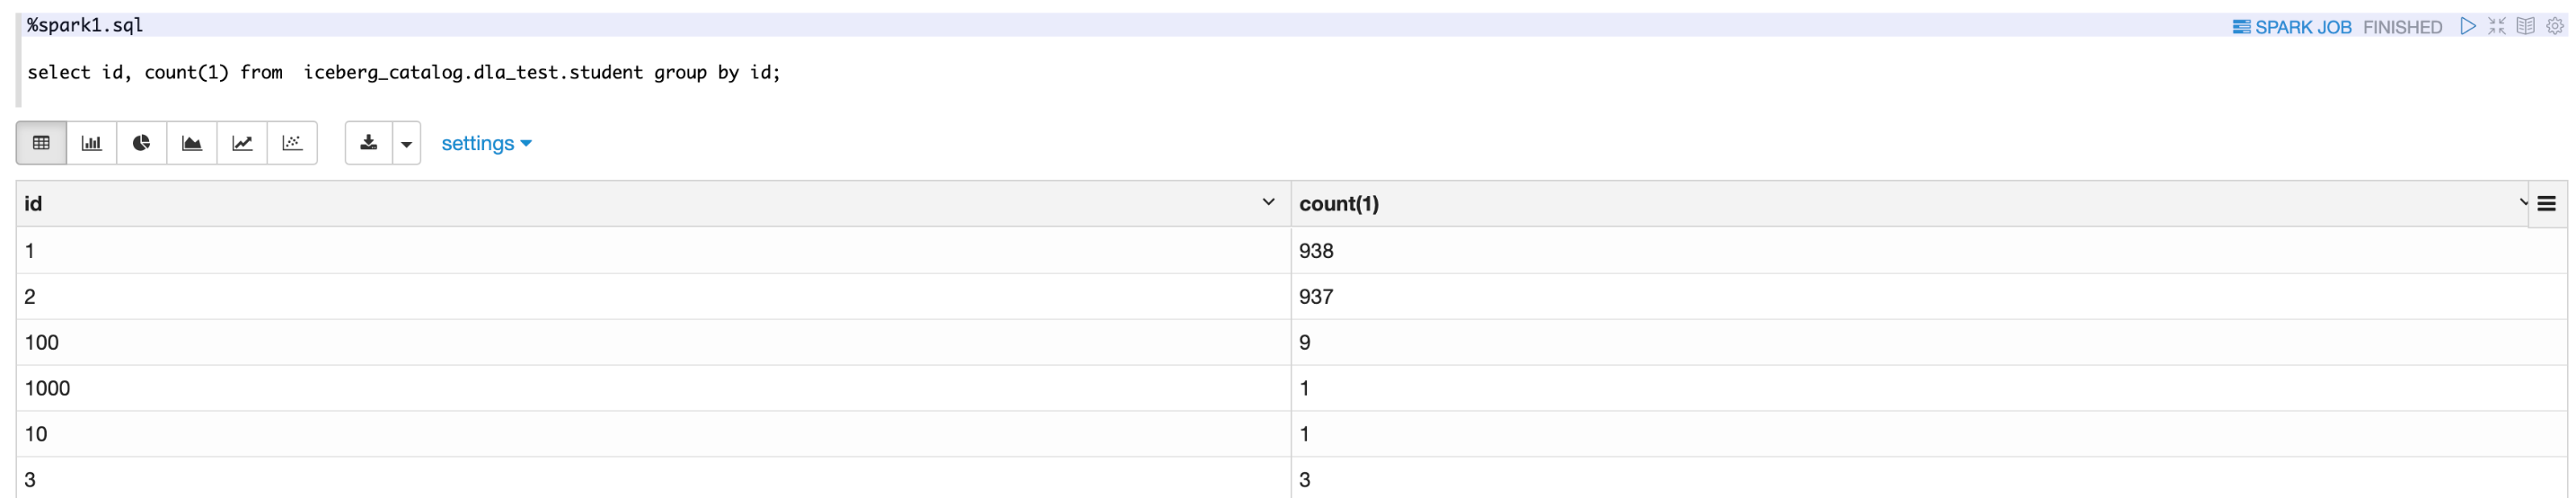
\includegraphics[width=1.0\textwidth]{zeppelin查询测试.png}
  \caption{Zeppelin查询测试}
  \label{fig:badge1}
\end{figure}

\section{自动优化服务}

自动优化服务是我们为了帮助用户一键启动优化,摆脱之前运维成本高而设计的。我们可以在元数据页面看到
每个表都有一个优化的按钮,通过此按钮我们可以配置并启动Iceberg表的自动优化,当前支持的优化有小文件合并、
历史快照清除、孤儿文件清除、生命周期管理。配置数据优化服务和停止服务的测试如表\ref{tab:exampletable13}和\ref{tab:exampletable14}所示:

\begin{table}[H]
  \centering
  \caption{配置数据优化服务接口测试}
  \label{tab:exampletable13}
  \begin{tabular}{ll}
    \toprule
    接口描述         & 配置数据优化服务         \\
    \midrule
    测试类型         & 功能测试         \\
    前置条件         & 后端服务器、MySQL服务器、Hive Metastore、US正常         \\
    接口地址       & /formation/v1/optimizer/configOptimizer        \\
    请求方式         & POST      \\
    请求数据类型         & application/json     \\
    响应数据类型         & application/json,*/*           \\
    实际结果         & 达到预期结果           \\
    结论            & 测试通过           \\
    \bottomrule
  \end{tabular}
\end{table}

\begin{table}[H]
  \centering
  \caption{停止数据优化服务接口测试}
  \label{tab:exampletable14}
  \begin{tabular}{ll}
    \toprule
    接口描述         & 停止数据优化服务         \\
    \midrule
    测试类型         & 功能测试         \\
    前置条件         & 后端服务器、MySQL服务器、Hive Metastore、US正常         \\
    接口地址       & /formation/v1/optimizer/disableService        \\
    请求方式         & POST      \\
    请求数据类型         & application/json     \\
    响应数据类型         & application/json,*/*           \\
    实际结果         & 达到预期结果           \\
    结论            & 测试通过           \\
    \bottomrule
  \end{tabular}
\end{table}

对于数据优化的效果,我们进行了表\ref{tab:exampletable15}的测试:

\begin{table}[H]
  \centering
  \caption{数据优化效果测试}
  \label{tab:exampletable15}
  \begin{tabular}{ll}
    \toprule
    测试描述         & 数据优化效果测试,均在默认参数设置下         \\
    \midrule
    用户场景         & 2min一个checkpoint,一次checkpoint产生50个2MB的小文件   \\
                   & 则一天会产生60 / 2 * 24 * 3=2000个元数据文件          \\
                   & 60 / 2 * 24 * 50=36,000个2MB的小文件              \\
                   & 按小时分区,数据保存30天,总大小2.16TB         \\
    不执行优化服务         & 元数据文件:2000 * 30 = 60000         \\
                        & 数据文件:36000 * 30=1080000个2MB的小文件         \\
    执行优化服务       & 元数据文件:约4700个(保留2天的快照文件和3天的metadata文件)        \\
                    & 数据文件:72000个2MB的小文件和21600个100MB的大文件        \\
    \bottomrule
  \end{tabular}
\end{table}

\section{性能测试}

本节主要对数据湖分析系统的性能进行测试,以元数据管理模块为例,使用JMeter对系统的主要接口进行压力测试\cite{33},
测试用例如下表\ref{tab:exampletable16}所示,测试结果如图\ref{fig:badge2}所示:

\begin{table}[H]
  \centering
  \caption{压力测试用例}
  \label{tab:exampletable16}
  \begin{tabular}{ll}
    \toprule
    测试描述         & 元数据管理模块性能测试         \\
    \midrule
    测试类型         & 性能测试         \\
    前置条件         & 用户成功登录系统         \\
    测试方法         & 使用JMeter模拟多用户进行压力测试        \\
    执行步骤         & 设置为1000个用户,每个用户访问10次,在60s内完成      \\
    预期结果         & 总共10000个请求,平均响应时间在500ms内,百分之95的响应在1s内      \\
    实际结果         & 达到预期结果           \\
    结论            & 测试通过           \\
    \bottomrule
  \end{tabular}
\end{table}

\begin{figure}[H]
  \centering
  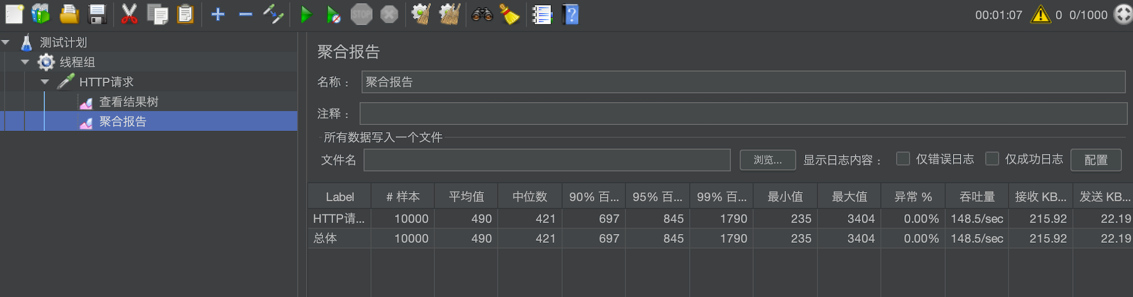
\includegraphics[width=1.0\textwidth]{压力测试结果.png}
  \caption{压力测试结果}
  \label{fig:badge2}
\end{figure}

\section{本章小结}

本章主要介绍了系统功能测试和性能测试。在系统功能测试中对系统各个
模块设计了大量的接口测试,并且根据测试结果对系统设计方案进行了改进,
本章只列举了部分关键接口测试。在系统性能测试中主要以元数据管理模块为例,
设计了压力测试用例,测试结果符合预期。
